\documentclass[ignorenonframetext]{beamer}

\useinnertheme[shadow=true]{rounded}
\useoutertheme{shadow}
\usecolortheme{orchid}
\usecolortheme{whale}

\date[05.02.2014]{February 5, 2014}

\usepackage[latin1]{inputenc}
\usepackage{listings}

\title{The Poisson problem - definition, applications and discretization}
\author{Arne Morten~Kvarving}
\subject{Numerical solution of PDEs}

\institute[SINTEF]{
  Department of Applied Mathematics\\
  SINTEF ICT}

\newcommand{\ub}[1]{\underbar{$#1$}\,}

\begin{document}

\frame{\maketitle}
\frame[label=example1]{
  \frametitle{The Poisson problem}
  \begin{itemize}
    \item The Poisson equation is an elliptic partial differential equation.
     \item The Poisson problem is the solution of the Poisson equation equipped with
           a set of boundary conditions.
     \item The equation is given by
       \begin{equation}
         -\nabla^2 u = f,\hspace{1cm} \text{ in } \Omega
       \end{equation}
       where $u$ is the unknown, $f$ is the load on the system and $\Omega$ denotes some domain.
     \item We remark that $\nabla^2$ is the sum of the second order partial derivatives, e.g.
       in 1D it reads
       \[
         -u_{xx} = f
       \]
       and in 2D it reads
       \[
         -(u_{xx} + u_{yy}) = f.
       \]
  \end{itemize}
}
\frame[label=example2]{
  \frametitle{The Poisson problem contd.}
  \begin{itemize}
    \item This equation is important for several reasons;
      \begin{enumerate}
        \item A number of physical processes are modelled directly by this equation.
        \item As a building block in modelling more complex processes.
      \end{enumerate}
     \item It models a diffusion process.
     \item Solution in the domain uniquely defined by the boundary data and the
       internal loads.
  \end{itemize}
}
\frame[label=example3]{
  \frametitle{Electrostatics}
  \begin{itemize}
    \item The differential forms for the electric field $\mathbf{E}$ are
      \[
        \begin{split}
          \nabla \cdot \mathbf{E} &= 4\pi\rho \\
          \nabla \times \mathbf{E} &= 0,
        \end{split}
      \]
      where $\rho$ is the charge density.
    \item The electric field $\mathbf{E}$ can be expressed as the gradient of
    a scalar potential $\Phi$, i.e. $\mathbf{E} = -\nabla\Phi$. Thus
    \[
      \nabla \cdot \mathbf{E} = -\nabla\cdot\nabla\Phi = -\nabla^2\Phi = 4\pi\rho.
    \]
  \end{itemize}
}
\frame[label=example4]{
  \frametitle{Potential flow}
  \begin{itemize}
    \item Likewise, potential flow in fluid mechanics can be modelled by this equation.
    \item Given a velocity field $\mathbf{U}$ which is irrotational and incompressible,
      \[
        \begin{split}
          \nabla \times \mathbf{U} &= 0 \\
           \nabla \cdot \mathbf{U} &= 0,
        \end{split}
      \]
      it follows that $\mathbf{U} = \nabla\Phi$ where $\Phi$ is a scalar velocity potential,
      which satisfies the Laplace equation
      \[
        \nabla^2\Phi = 0.
      \]
  \end{itemize}
}
\frame[label=example5]{
  \frametitle{Steady heat transfer}
  \begin{itemize}
    \item Energy transfered out of an arbitrary domain $\Omega$ can be expressed as
      \[
        \int_{\partial\Omega} \mathbf{q}\cdot\mathbf{n}\,\mathrm{d}S = \int_\Omega f\,\mathrm{d}\Omega.
      \]
      where $\mathbf{q}$ is the heat flux, $\mathbf{n}$ is the outward surface normal along
      the boundary $\partial\Omega$ and $f$ represents a volumetric heat source.
      This basically says that the net energy generation inside the domain must equal the net
      energy flowing out of the domain.
    \begin{figure}[H]
      \begin{center}
        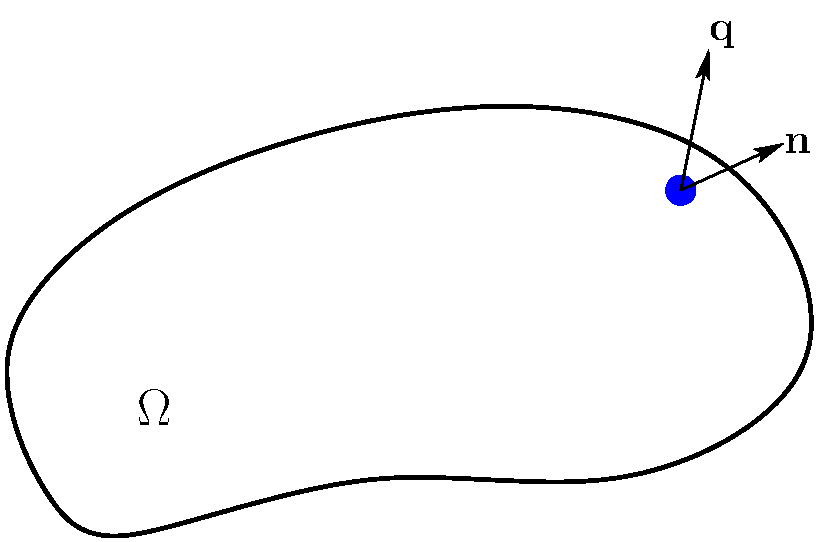
\includegraphics[width=4cm]{../../notes/06.poisson/HeatFlux}
      \end{center}
    \end{figure}
  \end{itemize}
}
\frame[label=example6]{
  \frametitle{Steady heat transfer contd.}
  \begin{itemize}
    \item Applying the Gauss' divergence theorem, we can write
      \[
        \int_{\partial\Omega}\mathbf{q}\cdot\mathbf{n}\,\mathrm{d}S = \int_\Omega \nabla \cdot \mathbf{q}\,\mathrm{d}\Omega = \int_\Omega f\,\mathrm{d}\Omega,
      \]
      yielding
      \[
        \nabla\cdot\mathbf{q} = f.
      \]
    \item Applying Fourier's law, i.e. $\mathbf{q} = -\kappa\nabla u, \kappa > 0$, we get
      \[
        \nabla\cdot\kappa\nabla u = f\hspace{1cm} \text{ in } \Omega,
      \]
      to be solved for the temperature $u$.
    \item For a constant heat conductivity $\kappa$, we regain the Poisson equation,
      \[
        \kappa\nabla^2 u = f.
      \]
  \end{itemize}
}
\frame[label=example7]{
  \frametitle{Unsteady heat transfer}
  \begin{itemize}
    \item Unsteady heat transfer is modelled by the heat equation
      \[
        \frac{\partial u}{\partial t} = \kappa\nabla^2u + f\hspace{1cm} \text{ in } \Omega.
      \]
    \item Discretizing in time using Backward Euler, we otain
      \[
        \frac{u^{n+1}-u^n}{\Delta t} = \kappa\nabla^2u^{n+1}+f^{n+1}
      \]
      where superscript n refers to a quanity at time $t^n, n=0,1,\cdots$.
    \item Can be rewritten as
      \[
        \left[-\kappa\nabla^2 + \frac{1}{\Delta t}\right]u^{n+1} = \frac{u^n}{\Delta t}+f^{n+1}.
      \]
    \item This is an \emph{Helmholtz} equation - Laplacian plus a multiple of the identity.
  \end{itemize}
}
\frame[label=example8]{
  \frametitle{Structural loads}
  \begin{itemize}
    \item Eigenmodes (eigenvibrations) in structures (bridges, buildings, turbines) are important in engineering.
    \item Want to design to avoid these for typical loads.
    \item To illustrate this, consider the eigenvalue problem
      \[
        -\nabla^2u = \lambda u
      \]
      where $u$ is the eigenmode and $\lambda$ the eigenvalue or frequency associated with the mode.
    \item The smallest eigenvalue/eigenmode pairs give information of physical importance.
  \end{itemize}
}
\frame[label=example10]{
  \frametitle{Solving PDEs on computers}
  \begin{itemize}
    \item Typically we can only solve the equation in an approximate sense.
    \item Computers can only work on finite-dimensional data.
    \item The process of approximating a continuous equation with a finite dimensional
      one is called \emph{discretizing} the equation.
    \item Several ways to do this.
    \item The most popular ones: \emph{finite differences}, \emph{finite volumes}, \emph{finite elements}.
  \end{itemize}
}
\frame[label=example11]{
  \frametitle{Solving PDEs on computers}
  \begin{itemize}
    \item This is not a course in discretization of PDEs.
    \item We will concentrate on the finite difference approach since it is the least
        technical.
    \item However, all of them have something in common: At the end of the day you
      end up with a set of linear equations to solve,
      \[
        \ub{A}\ub{u} = \ub{g}
      \]
      where $\ub{A}$ is the matrix of linear equations, $\ub{u}$ the unknown solution
      and $\ub{g}$ the discretized load on the system (the right hand side).
    \item We will focus mostly on solving the equations, and thus most of what we consider
      is applicable no matter the discretization approach.
  \end{itemize}
}
\frame[label=example12]{
  \frametitle{Finite difference methods}
  \begin{itemize}
    \item Consider a continuous function 1D function $u(x)$.
    \item Introduce a grid, $\left\{x_i\right\}_{i=0}^N$, with $x_i = x_0+ih$.
    \item Here $h$ is the grid spacing. For simplicity we consider equidistant grids (constant $h$).
    \begin{figure}[H]
      \begin{center}
        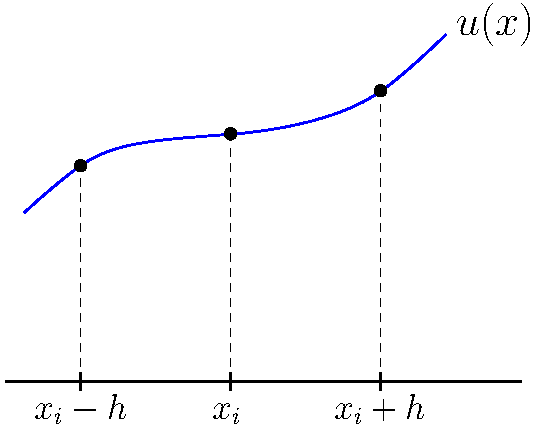
\includegraphics[width=4cm]{../../notes/07.poisson-fdm/FiniteDifference}
      \end{center}
    \end{figure}
    \item Want to approximate derivatives of the function only using data on the grid.
  \end{itemize}
}
\frame[label=example13]{
  \frametitle{Finite difference methods}
  \begin{itemize}
    \item First idea: How derivatives were introduced in high school:
      \[
        u'\left(x_i\right) \approx \frac{u\left(x_i+h\right)-u\left(x_i\right)}{h}.
      \]
    \item This is called a one-sided difference. Invoking Taylor we find
      \[
        \begin{split}
          \frac{u\left(x_i+h\right)-u\left(x_i\right)}{h} &= \frac{u\left(x_i\right) + hu'\left(x_i\right) + \frac{h^2}{2}u''\left(x_i\right) -u\left(x_i\right)}{h} \\
                                                          &= u'\left(x_i\right) + \mathcal{O}(h).
        \end{split}
      \]
      In other words, this is a \emph{first order} approximation to $u'\left(x_i\right)$.
  \end{itemize}
}
\frame[label=example14]{
  \frametitle{Finite difference methods}
  \begin{itemize}
    \item Second idea: A centered difference
      \[
        u'\left(x_i\right) \approx \frac{u\left(x_i+h\right)-u\left(x_i-h\right)}{2h}.
      \]
    \item Invoking Taylor we find
      \[
        \begin{split}
          \frac{u\left(x_i+h\right)-u\left(x_i-h\right)}{2h} &= u'\left(x_i\right) + \mathcal{O}\left(h^2\right).
        \end{split}
      \]
      In other words, this is a \emph{second order} approximation to $u'\left(x_i\right)$.
  \end{itemize}
}
\frame[label=example15]{
  \frametitle{Finite difference methods}
  \begin{itemize}
    \item A centered difference for the second derivative:
      \[
        u''\left(x_i\right) \approx \frac{u'\left(x_i+\frac{h}{2}\right)-u'\left(x_i-\frac{h}{2}\right)}{h}.
      \]
    \item Invoking Taylor we find
      \[
        \begin{split}
          \frac{u'\left(x_i+\frac{h}{2}\right)-u'\left(x_i-\frac{h}{2}\right)}{h} &=  \\
                 \frac{u\left(x_i-h\right)+u\left(x_i+h\right)-2u\left(x_i\right)}{h^2} &= u''\left(x_i\right) + \mathcal{O}\left(h^2\right).
        \end{split}
      \]
      In other words, this is a \emph{second order} approximation to $u''\left(x_i\right)$.
    \item Can be visualized by the stencil
    \begin{center}
      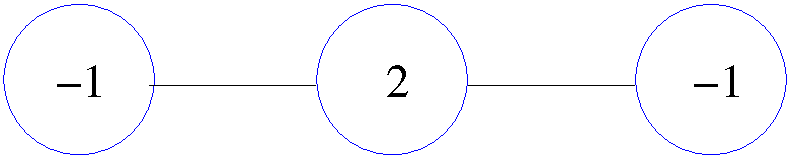
\includegraphics[width=4cm]{../../notes/07.poisson-fdm/ThreePointStencil}
      \end{center}
    (here the stencil for $-u_{xx}$).
  \end{itemize}
}
\frame[label=example16]{
  \frametitle{Discretizing the 1D Poisson problem}
  \begin{itemize}
    \item We now consider the 1D Poisson problem
      \[
        \begin{split}
          -u_{xx} &= f, \hspace{1cm} \text{ in } \Omega = (0,1), \\
           u(0) &= u(1) = 0.
        \end{split}
      \]
      \begin{center}
        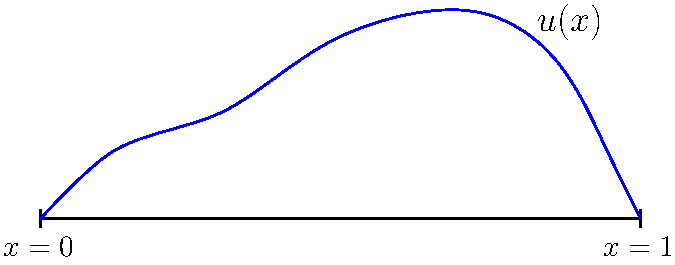
\includegraphics[width=4cm]{../../notes/07.poisson-fdm/Poisson1D_Domain}
      \end{center}
    \item These are called homogenous Dirichlet boundary conditions - 
          solution is prescribed to be 0 on the boundaries of the domain.
    \item Introduce the grid, $\left\{x_i\right\}_{i=0}^N$, with $x_i = x_0+ih$, $h = \frac{1}{N}$.
      \begin{center}
        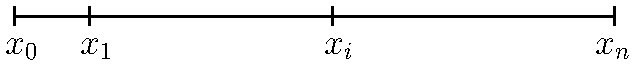
\includegraphics[width=4cm]{../../notes/07.poisson-fdm/Poisson1D_Grid}
      \end{center}
  \end{itemize}
}
\frame[label=example17]{
  \frametitle{Discretizing the 1D Poisson problem contd.}
  \begin{itemize}
    \item Let $u_i$ denote $u\left(x_i\right)$ and $f_i$ denote $f\left(x_i\right)$.
    \item Due to the boundary conditions we know that $u_0 = u_N = 0$.
    \item We thus have $N-1$ unknowns. We collect these in a vector $\ub{u}$.
    \item We then apply the second order finite difference formula in each grid point.
    \begin{align*}
      -\left( \frac{u_{i+1} - 2u_i + u_{i-1}}{h^2} \right) &= f_i, \qquad i=1,\ldots,n-1, 
      u_0 &= 0, \\
      u_{n} &= 0.
    \end{align*}
  \end{itemize}
}
\frame[label=example18]{
  \frametitle{Discretizing the 1D Poisson problem contd.}
  \begin{itemize}
    \item The equations can also be expressed as the system
      \begin{align*}
        2 u_1 - u_2 &= h^2 f_1, \\
        -u_1 + 2 u_2 - u_3 &= h^2 f_2, \\
        &\vdots \\
        -u_{n-2} + 2 u_{n-1} &= h^2 f_{n-1}.
      \end{align*}
      We have here already used the fact that $u_0=0$ and $u_{n}=0$.
    \item Or in matrix form;
      \begin{align*}
       \underbrace{ \begin{bmatrix}
          2 & -1 & & & \\
          -1 & 2 & -1 & & \\
          & & \ddots & & \\
          & & -1 & 2 & -1 \\
          & & & -1 & 2
        \end{bmatrix}
        }_{\underline{A}}
        \underbrace{ \begin{bmatrix}
          u_1 \\
          u_2 \\
          \vdots \\
          u_{n-2} \\
          u_{n-1}
        \end{bmatrix}
        }_{\underline{u}}
        &= 
        \underbrace{h^2 \begin{bmatrix}
          f_1 \\
          f_2 \\
          \vdots \\
          f_{n-2} \\
          f_{n-1}
        \end{bmatrix}
        }_{\underline{g}}.
      \end{align*}
  \end{itemize}
}
\frame[label=example19]{
  \frametitle{Discretizing the 1D Poisson problem contd.}
  \begin{itemize}
    \item The matrix $\ub{A}$ is sparse (tridiagonal).
    \item The matrix $\ub{A}$ is symmetric, that is $\ub{A} = \ub{A}^T$.
    \item The matrix $\ub{A}$ is positive definite, that is, 
          $\underline{v}^T \underline{A}\, \underline{v} > 0$ 
          for all vectors $\underline{v}\in \mathbb{R}^{n-1}$, $\underline{v} \not= \underline{0}$).
    \item Thus, the system of $n-1$ equations is solvable and has a unique solution.
    \item The error in the grid points is of second order, i.e. $|u(x_i)-u_i| \sim \mathcal{O}(h^2)$.
  \end{itemize}
}
\frame[label=example20]{
  \frametitle{Discretizing the 1D Poisson problem contd.}
  \lstinputlisting[language=Matlab,basicstyle=\tiny]{poisson1D.m}
  \lstinputlisting[language=Matlab,basicstyle=\tiny]{source1.m}
  \lstinputlisting[language=Matlab,basicstyle=\tiny]{conv1.m}
}
\frame[label=example21]{
  \frametitle{Discretizing the 2D Poisson problem}
  \begin{itemize}
    \item We now consider the 2D Poisson problem.
      \[
        \begin{split}
          -\nabla^2 u &= f, \hspace{1cm} \text{ in } \Omega = \left(0,L_x\right)\times\left(0,L_y\right), \\
          u &= 0 \hspace{1cm} \text{ in } \partial\Omega.
        \end{split}
      \]
      \begin{center}
        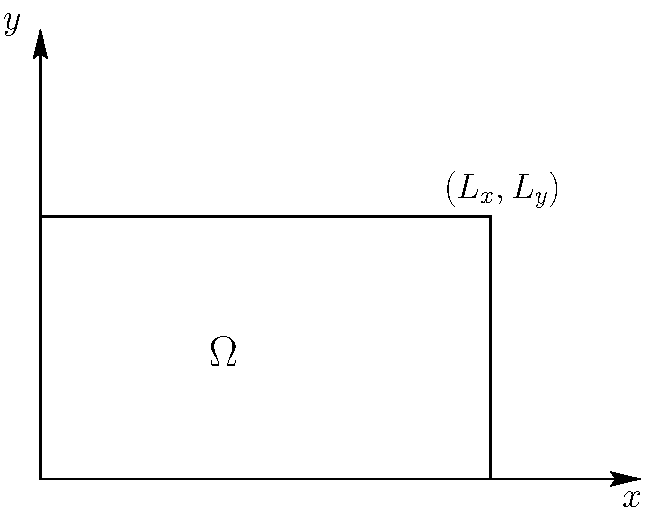
\includegraphics[width=3cm]{../../notes/07.poisson-fdm/Poisson2D_Domain}
      \end{center}
    \item Introduce the grid, $\left\{x_{i,j}\right\}_{i,j=0}^N$, with $x_{i,j} = \left(x_0+ih_x, y_0+ih_y\right)$, $h_x = \frac{L_x}{N}, h_y = \frac{L_y}{N}$.
      \begin{center}
        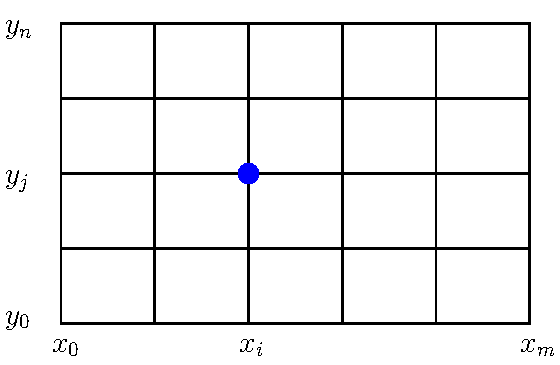
\includegraphics[width=3cm]{../../notes/07.poisson-fdm/Poisson2D_Grid}
      \end{center}
  \end{itemize}
}
\frame[label=example22]{
  \frametitle{Discretizing the 2D Poisson problem contd.}
  \begin{itemize}
    \item Let $u_{i,j} = u(x_i, y_j)$. We then have two differences;
      \begin{align*}
        \frac{u_{i+1,j} - 2 u_{i,j} + u_{i-1,j}}{h_x^2} &\simeq \left( \frac{\partial^2 u}{\partial x^2} \right) \biggl|_{(x_i,y_j)} + \quad\mathcal{O}(h_x^2), \\
        \frac{u_{i,j+1} - 2 u_{i,j} + u_{i,j-1}}{h_y^2} &\simeq \left( \frac{\partial^2 u}{\partial y^2} \right) \biggl|_{(x_i,y_j)} + \quad\mathcal{O}(h_y^2).
      \end{align*}
    \item For simplicity we assume $L_x = L_y$ in the following and thus
      $h_x = h_y = h$.
    \item Plugging this into our partial differential equation, we get
      \begin{align*}
        -u_{i+1,j}-u_{i-1,j}-u_{i,j+1}-u_{i,j-1}+4u_{i,j} &= h^2 f_{i,j}, i,j=1,\ldots,N-1.
      \end{align*}
  \end{itemize}
}
\frame[label=example23]{
  \frametitle{Discretizing the 2D Poisson problem contd.}
  \begin{itemize}
    \item Each point couple to their 4 neighbors (NSEW); five point stencil
      \begin{center}
        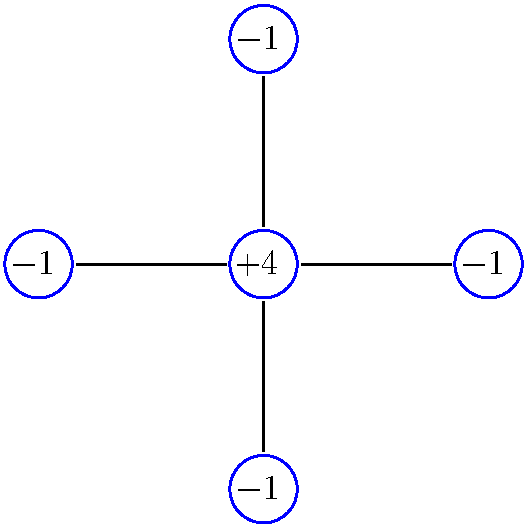
\includegraphics[width=4cm]{../../notes/07.poisson-fdm/FivePointStencil}
      \end{center}
  \end{itemize}
}
\frame[label=example24]{
  \frametitle{Discretizing the 2D Poisson problem contd.}
  \begin{itemize}
    \item We need a numbering scheme - in order to form the linear system
      of equations.
    \item We here use a natural, global numbering scheme; we number row by row.
      \begin{center}
        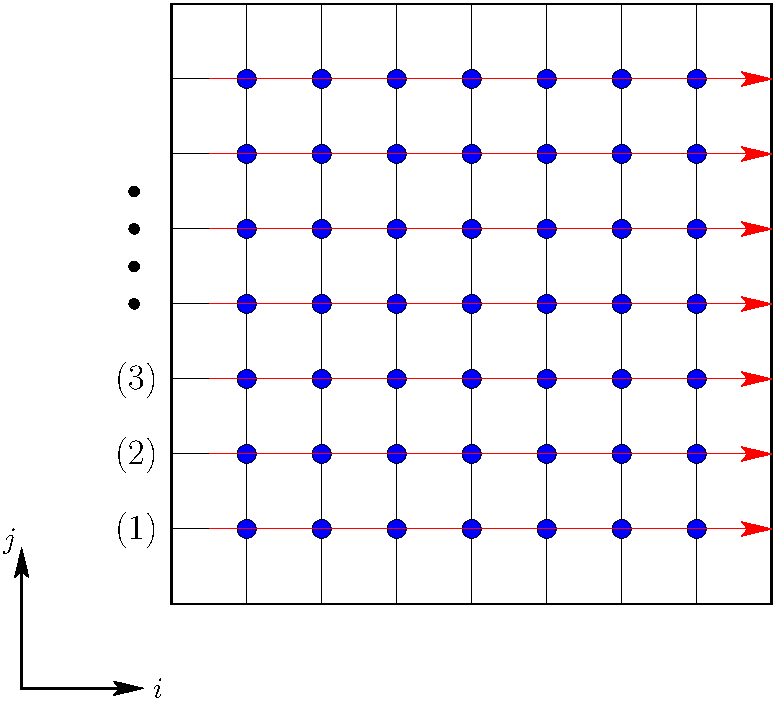
\includegraphics[width=3cm]{../../notes/07.poisson-fdm/NaturalOrdering}
      \end{center}
    \item Structure of equation system dependent on numbering scheme chosen.
  \end{itemize}
}
\frame[label=example25]{
  \frametitle{Discretizing the 2D Poisson problem contd.}
  \begin{itemize}
    \item With the chosen numbering scheme, we get the following linear
      system.
      \begin{center}
        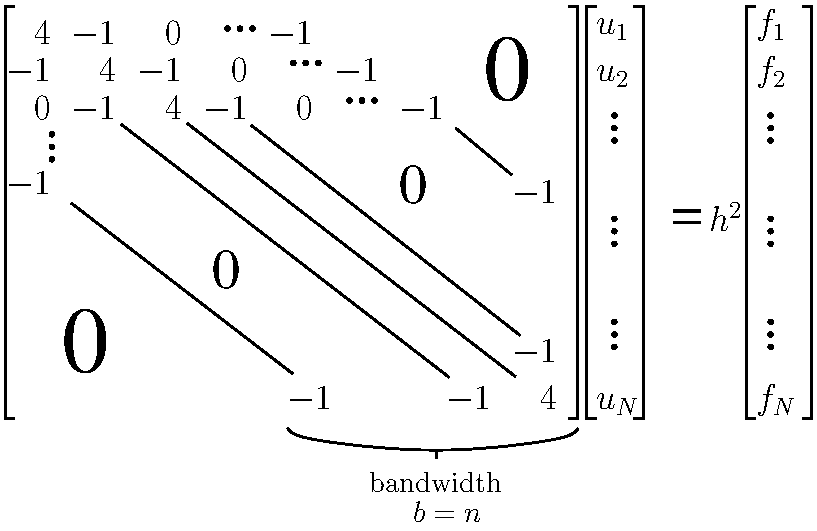
\includegraphics[width=8.5cm]{../../notes/07.poisson-fdm/Poisson2D_System}
      \end{center}
  \end{itemize}
}
\frame[label=example26]{
  \frametitle{Discretizing the 2D Poisson problem contd.}
  \lstinputlisting[language=Matlab,basicstyle=\tiny]{poisson2D.m}
  \lstinputlisting[language=Matlab,basicstyle=\tiny]{source2.m}
  \lstinputlisting[language=Matlab,basicstyle=\tiny]{conv2.m}
}
\end{document}
